
\documentclass[11pt,a4paper]{article}
\usepackage[hyperref]{naaclhlt2019}
\usepackage{times}
\usepackage{latexsym}
\usepackage{graphicx}
\usepackage[normalem]{ulem}

\usepackage[utf8]{inputenc} % allow utf-8 input
\usepackage[T1]{fontenc}    % use 8-bit T1 fonts
\usepackage{hyperref}       % hyperlinks
\usepackage{url}            % simple URL typesetting
\usepackage{booktabs}       % professional-quality tables
\usepackage{amsfonts}       % blackboard math symbols
\usepackage{nicefrac}       % compact symbols for 1/2, etc.
\usepackage{microtype}      % microtypography
\usepackage{indentfirst}
\usepackage{soul}

%\usepackage{layout}

% \setlength{\voffset}{-0.75in}
% \setlength{\headsep}{5pt}

\usepackage{url}

\aclfinalcopy 


\title{Survey of RNN-Attention Machine Translation Methods}

\author{Stephen Dong  \\
  {\tt stdong@ucsd.edu}\\
  {\tt June 7, 2024} \\}
  % Second Author \\
  % {\tt email@domain} \\\And
  % Third Author \\
  % {\tt email@domain} \\\And
  % Fourth Author \\
  % {\tt email@domain} \\}
  
% \setlength\textwidth{16.0cm}

\date{June 7, 2024}
\begin{document}
\maketitle

% \begin{abstract}
% \end{abstract}

 
% \section{Instructions}
%   {\color{blue}
%  \begin{itemize}
%      \item \textit{Length: Should be at least \textbf{5 pages} but not more than 8 pages. {Do not include this template content in your final report as it messes up page count}. 
%       Comment out everything in this document (except the headings when necessary)}
          
%      \item \textit{Submit (report, and optional code):  on Gradescope by \textbf{Friday, June 7, 2024}.}
%  \end{itemize} 
%  }

\section{Introduction}
% Original before both GPT proofread (this also includes any personal changes to information that might've been included after proofreaing that was not passed into GPT)
% This survey paper will focus on the analysis of neural machine translation (NMT). Machine Translation (MT) is a powerful automation tool to bridge the gap between languages by providing end-to-end translation between two languages. Translation tools like Google Translate have been an integral part of our society for the past few decades. Early MT tools have primarily been utilized to translate words and eventually simple phrases, but were still relatively inaccurate with more complex linguistics and sentences \cite{WANG2022143}. 

% Early MT approaches relied on rule-based methods; however, these approaches were tedious as they required manual translation from a dictionary. The 1990s saw the initial proposal of corpus-based statistical machine translation (SMT) models. Phrase-based SMT methods were later introduced in 2003 with "Pharaoh" and "Moses" as the primary innovations. \cite{WANG2022143} 

% Simple SMTs remained the dominant implementation of MT models until Nal Kalchbrenner, et al. \cite{kalchbrenner-blunsom-2013-recurrent} proposed the first NMT model that used an encoder-decoder structure for end-to-end translation. The paper proposed the recurrent continuous translation model (RCTM), which uses a convolutional neural network (CNN) in the encoder and an inverted CNN followed by a recurrent neural network (RNN) for the decoder. 

% Following this proposal, KyungHyun Cho et al. reveals a seperate alternative approach similar to Kalchbrenner's RCTM model that also incorporates the RNN into the encoder \cite{cho2014learning}. The paper also proposed a faster variation of the long-short term memory (LSTM) hidden unit, later denoted as a gated recurrent unit (GRU), to solve issues with retaining distant relevant information in longer sentences, allowing for higher BLEU scores as shown in Figure 1.

% The proposed GRU contains two primary gates: reset and update, shown in Figure 2. The update gate controls what new information from the new hidden state should be included in the hidden state. Meanwhile, the reset gate drops any information that displays signs of irrelevancy. These gates allow the unit to mimic long-term and short-term memory, i.e. long-term memory has more update gate activations and short-term memory with reset gates activations. \cite{cho2014learning} These gates allow the GRU to capture information in more meaningfully ways to boost performance.

% The models presented in both papers served as the backbone of future NMT models. The following years introduced the use of attention in MT models, with Google pushing out their state-of-the-art GNMT model for Google Translate \cite{wu2016googles}. The same year, Dzmitry Bahdanau et al. published their paper Neural Machine Translation By Jointly Learning to Align and Translate \cite{bahdanau2016neural}, which adds an attention mechanism to the GRU encoder-decoder model proposed by Cho.

% This survey will explore the attention-based RNN encoder-decoder model presented by Bahdanau et al. \cite{bahdanau2016neural}. This approach adds an attention mechanism in the decoder and converts the uni-directional encoder into a bi-directional RNN to extract and retain information behind and in front of each token. The paper suggests the model is capable of achieving an increased BLEU score of any long sentence translations.

% This paper will demonstrate the continued limitations of the attention RNN encoder-decoder model with longer and more complex, or rather realistic, sentence structures. This is an important consideration as recent increases in tourism around the world have prompted the need for accurate translations of large passages all at once. The codebase used for this survey is a smaller scaled tutorial implementation of the PyTorch seq2seq module \cite{github}. This codebase was also chosen for its accurate reflection of the model presented by the paper, but scaled down for hardware limitations. Results presented in this survey will be analyzed with this consideration. The BLEU scores of the test set of the original codebase's dataset for the attention RNN encoder-decoder model will serve as a baseline..

% After GPT Proofread
This survey paper will focus on the analysis of neural machine translation (NMT). Machine Translation (MT) is a powerful automation tool to bridge the gap between languages by providing end-to-end translation between two languages. Translation tools like Google Translate have been an integral part of our society for the past few decades. Early MT tools primarily translated words and eventually simple phrases but were still relatively inaccurate with more complex linguistics and sentences \cite{WANG2022143}.

Early MT approaches relied on rule-based methods; however, these approaches were tedious as they required manual translation from a dictionary. The 1990s saw the initial proposal of corpus-based statistical machine translation (SMT) models. Phrase-based SMT methods were later introduced in 2003 with "Pharaoh" and "Moses" as the primary innovations, but these could only accurately translate smaller phrases. \cite{WANG2022143}

SMTs remained the dominant implementation of MT models until Nal Kalchbrenner, et al. \cite{kalchbrenner-blunsom-2013-recurrent} proposed the an NMT model that used an encoder-decoder structure for end-to-end translation. The paper proposed the recurrent continuous translation model (RCTM), which uses a convolutional neural network (CNN) in the encoder and an inverted CNN followed by a recurrent neural network (RNN) for the decoder.

Following this proposal, KyungHyun Cho et al. revealed a separate alternative approach similar to Kalchbrenner's RCTM model that also incorporates the RNN into the encoder \cite{cho2014learning}. The paper also proposed a faster variation of the long-short term memory (LSTM) hidden unit, later denoted as a gated recurrent unit (GRU), to solve issues with retaining distant relevant information in longer sentences, allowing for higher BLEU scores as shown in Figure 1.

\begin{figure}[h]
    \centering
    % \includegraphics[width=0.475\linewidth]{figures/LM_Default_Dropout/LM_Loss_Dropout.png}
    % \includegraphics[width=0.475\linewidth]{figures/LM_Default_Dropout/LM_Per_Dropout.png}
    \begin{tabular}{| l || c |}
    \hline
    Model & BLEU Test\\
    \hline
    \hline
    RCTM I + WP & 21.5\\
    RCTM II + WP & 21.7\\
    \hline
    RNN & 33.87\\
    CSLM + RNN & 34.64\\
    CSLM + RNN + WP & 34.54\\
    \hline
    \end{tabular}
    \caption{Side-by-side BLEU test results comparison of RCTMs \cite{kalchbrenner-blunsom-2013-recurrent} with word penalty (WP) and RNN and LSTM based encoder-decoder and semantic retention models with and without WP \cite{cho2014learning}}
\end{figure}

The proposed GRU contains two primary gates: reset and update, shown in Figure 2. The update gate controls what new information from the new hidden state should be included in the hidden state. Meanwhile, the reset gate drops any information that displays signs of irrelevancy. These gates allow the unit to mimic long-term and short-term memory, i.e. long-term memory has more update gate activations and short-term memory with reset gates activations. \cite{cho2014learning} These gates allow the GRU to capture information in more meaningfully ways to boost performance.

\begin{figure}[h]
    \centering
    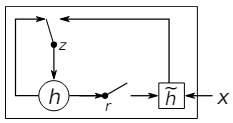
\includegraphics[]{figs/GRU_hidden_cell.png}
    \caption{GRU illustration from Cho et al.'s paper \cite{cho2014learning} with $z$ as the update gate, $r$ as the reset gate, $h$ as the current hidden state, and $\widetilde{h}$ as the new hidden state with new $x$ information.} 
\end{figure}

The models presented in both papers served as the backbone of future NMT models. The following years introduced the use of attention in MT models, with Google pushing out their state-of-the-art GNMT model for Google Translate \cite{wu2016googles}. The same year, Dzmitry Bahdanau et al. published their paper \textit{Neural Machine Translation By Jointly Learning to Align and Translate} \cite{bahdanau2016neural}, which adds an attention mechanism to the GRU encoder-decoder model proposed by Cho.

This survey will explore the attention-based RNN encoder-decoder model presented by Bahdanau et al. \cite{bahdanau2016neural}. This approach adds an attention mechanism in the decoder and converts the unidirectional encoder into a bidirectional RNN to extract and retain information behind and in front of each token. The paper suggests the model is capable of achieving an increased BLEU score of any long sentence translations. 

This paper will demonstrate the continued limitations of the attention RNN encoder-decoder model with longer and more complex, or rather realistic, sentence structures. This is an important consideration as recent increases in tourism around the world have prompted the need for accurate translations of large passages all at once. The codebase used for this survey is a smaller scaled tutorial implementation of the PyTorch seq2seq module \cite{github}. This codebase was also chosen for its accurate reflection of the model presented by the paper, but scaled down for hardware limitations. Results presented in this survey will be analyzed with this consideration. The BLEU scores of the test set of the original codebase's dataset for the attention RNN encoder-decoder model will serve as a baseline.

% \textbf{Task and Model Summary}: Briefly summarize the NLP \textbf{problem or task} chosen and explain its importance. Specify the \textbf{model or system} selected, including references to the paper and the source code. (It is fine if  your task is different from the one in your proposal.)

% \noindent \textbf{Approach and Findings Summary}: Describe the approach taken for analyzing the system. Summarize the main limitations identified during the analysis.


\section{The Dataset and Model}
\subsection{Training}
The original dataset \cite{elliott-EtAl:2016:VL16} provided by the codebase is used to train a model for German-English translations. The dataset contains a much smaller set of approximately 32K sentence translations of approximately 400K words compared to the approximately 348M words of the original paper \cite{bahdanau2016neural}. 20,518,405 parameters are learnable during training and is validated on 1,014 en-de translations. 1,000 en-de translations are used to test the capabilities of the model. All preprocessing and model implementations will be the default provided by the codebase.

This dataset is loaded in from Huggingface\footnote{https://huggingface.co/datasets/bentrevett/multi30k} into a \verb|Dataset| from Huggingface's datasets module. Each sentence is tokenized and \verb|<sos>| and \verb|<eos>| tokens are prepended and appended to each sentence, respectively. The vocabulary for both German and English is built using the training data. Words that only occur once are filtered out as no meaningful information can be obtained from them besides the sentences they appeared in. The indices of each token in respect to the vocabulary is generated for the training, validation, and testing data. Given that the data is in \verb|Dataset| objects, each data must also be formatted for PyTorch. 

Both the encoder and decoder have an embedding dimension of $256$ and a hidden dimension of $512$ in substitution of the 620 embedding dimensionality and 1000 hidden units suggested by original paper. The encoder and decoder uses the GRU module in PyTorch. Note that \verb|tanh| is used as the activation function as suggested by the paper. A dropout of $p=0.5$ is also applied to both the encoder and decoder to serve as regularization for only this codebase. 

A batch size of $128$ is used to collate and form the dataloaders to train, evaluate, and test the model. The weights are initialized with Gaussian normal values and adjusted with the Cross-Entropy loss function during training. The model will be trained for 10 epochs using the \verb|Adam| optimizer with default PyTorch parameters ($lr=0.001, \beta_1=0.9, \beta_2=0.999, \epsilon=1e-8$). The training, validation, and testing will be performed on a single 32GB Cuda-enabled GPU (Nvidia RTX2080 Super).

\subsection{Extreme Stress Test Dataset}
The \textit{wmt\_t2t} dataset \cite{bojar-EtAl:2014:W14-33} will be used to test the model against a larger corpus databases with more extreme entries. This dataset is pulled from Huggingface\footnote{https://huggingface.co/datasets/wmt/wmt\_t2t} and will contain a train, validation, and test split of 4592289, 3000, and 3003 rows of single or multiple sentences. However, due to hardware limitations, only about $5\%$ of each split of the dataset ($229614$ train, $150$ validation, and $150$ test rows for a total of $229914$ rows) will be used to prevent the GPU from running out of memory during testing. Rows that are included into the test set will randomly be selected from each split with uniform probability. The dataset will be preprocessed in the same way as the training dataset to be used in the translation model. 

The purpose of this dataset is to test the model against a large set of entries that may be more complex and extreme in context and length. These entries are used to mimic potential real-life use cases where an entire page is translated at once such that references, notices, or non-conversational text in German may also need to be translated. One such expected de-en translation example of this extreme case is shown:

\begin{center}
\begin{tabular}{p{2.5in}}
    \hline
    b4 - 0295 / 96 - 0 - 0071 / 96 der abgeordneten Burenstam Linder und Martens im namen der ppe-fraktion an den rat\\
    \\
    by Mr Burenstam Linder and Mr Martens, on behalf of the Group of the European People's Party, to the Council (B4-0295/96 - O-0071/96)\\
    \hline
    \\
    \textit{Note: This is cropped for brevity. The original de-en sentences have \~333 words.}
\end{tabular}
\end{center}

Moreover, these entries contain more realistic writings one may expect from a webpage or reading as shown in the English comparison with an entry of the training dataset:

\begin{center}
\begin{tabular}{p{2.5in}}
    Training:\\
    \hline
    Man on skis looking at artwork for sale in the snow.\\
    A black dog stands on top of a brown dog on the grass.\\
    \hline
    \\
    "Real" writing from extreme dataset:\\
    \hline
    My question relates to something that will come up on Thursday and which I will then raise again.\\
    \hline
\end{tabular}
\end{center}

\subsection{Manageable Stress Test Dataset}
An open-source \textit{manageable} stress test dataset from the Tatoeba Project\footnote{Downloaded from https://www.manythings.org/anki/} \cite{anki} will also be used to analyze the model's capability in translating a range of sentence lengths and complexity. This dataset contains about $277891$ sentences varying between 1 to approximately 75 words, making it slightly more maneagable for the model to translate. The dataset must be read from a tab-separated text file and converted into a \verb|Dataset| object with the same \verb|en| and \verb|de| columns to be preprocessed to be usable by the translation model. This dataset is meant to stress test the model with both extremely low and high count sentences and analyze if it can perform well with longer sentences that are small enough to be optimistic of results. It should be noted that the more complex, and consequently longer, entries share the same realistic writing style as the extreme dataset, for example:
\begin{center}
\begin{tabular}{p{2.5in}}
    \hline
    I could tell by the look on Tom's face that he knew what was going on.\\
    \hline
\end{tabular}
\end{center}

% The most important rule of NLP: look at your data! Describe the datasets used for analysis, including any preprocessing steps. This can be existing datasets used in the original paper, or it can be your own adversarial examples meant to stress test the system or it can be any benchmark datasests  such as those found on Huggingface datasets.

% Explain what properties of the data make it  challenging. Report  basic statistics (e.g., size, number of words/sentences/documents) and some other statistics that are specifically relevant to your task. Show a couple input / output pairs to make it clear what you're doing (but don't use up too much space in doing so.).

\section{Analysis Approach}
For both test datasets, the BLEU score from testing is reported and analyzed. The BLEU score is collectively computed with all of the generated de-en translations using the all of the input's true de-en translations as reference. Translation results are filtered out if the percentage of translated \verb|<unk>| tokens exceeds $25\%$ of the entire translation. These translations are automatically considered to have failed to translate under these extreme conditions. The unfiltered translations are considered "\textit{possibly} acceptable" and are further analyzed for performance. 

These translations will be sorted with attention maps generated according to each of these criteria: (1) most non-\verb|<unk>| tokens generated, (2) most unique non-\verb|<unk>| tokens generated. Criterion (1) is to analyze the behavior of the model when translating \textit{large} inputs (multiple or long sentences), particularly how well it was able to learn context from the input to generate translations. Criterion (2) is to analyze the quality of the translations as higher unique generations are more likely to contain better translations.

\begin{center}
\begin{tabular}{p{2.5in}}
    An example of a filtered translation:\\
    \hline
    \verb|<sos>| \verb|<unk>| a \verb|<unk>| \verb|<unk>| \verb|<unk>| \verb|<unk>| \verb|<unk>| \verb|<unk>| . \verb|<eos>|\\
    \hline
\end{tabular}
\end{center}

\begin{center}
\begin{tabular}{p{2.5in}}
    An example of a \textbf{poor} translation that was kept and considered \textit{possibly} acceptable:\\
    \hline
    \verb|<sos>| \verb|<unk>| throughout \verb|<unk>| throughout \verb|<unk>| throughout throughout throughout throughout throughout throughout throughout \verb|<eos>|\\
    \hline
\end{tabular}
\end{center}

\begin{center}
\begin{tabular}{p{2.5in}}
    An example of a \textbf{good} translation that was kept and considered \textit{possibly} acceptable:\\
    \hline
    \verb|<sos>| this long - haired \verb|<unk>| with their eyes closed on a a stand , one of them . \verb|<eos>|\\
    \hline
\end{tabular}
\end{center}

Each sentence of the manageable stress dataset is also categorized into four "complexity" groups. These groups are made by collecting the word count in the German sentence and given a number 1-4 based on these rules: [1] 1-24 words, [2] 25-49 words, [3] 50-74 words, [4] 75-99 words. Complexity groups 1 and 2 are expected to perform the best as they fall in the maximum tested sentence lengths of the paper. Sentences not in complexity group 1 bypass the filter for this dataset in order to analyze the performance of these longer sentences. Moreover, without this bypass, sentences in complexity groups 3 and 4 were all filtered out, which itself reveals the limitation of the model. 

Each translation is given a maximum word translation count of $1.5\times$ the input German sentence word count to account for possible additional word usage across languages. This also allows observations of how the model will translate the input given more space to generate words. The top sentence translations of each criteria mentioned will be analyzed along with the attention map it generates. 

% Explain the methods used to analyze the system. Tell us any interesting aspects about your approach.  This section can be pretty straightforward. However,  you are encouraged to explore systematic diagnostic methods if you feel inspired.  

\section{Errors and their Categorization}
\subsection{BLEU Results}

\begin{figure}[h]
    \centering
    \begin{tabular}{| l || c | c |}
    \hline
    Stress Dataset & Extreme & Manageable\\
    \hline
    Tr. Length & 10377756 & 4619553\\
    \hline
    Ref. Length & 6011421 & 2150004\\
    \hline
    BLEU & 0.0008996 & 0.0068542\\
    \hline
    \hline
    \hline
    \hline
    & Normal Dataset &\\
    \hline
    Tr. Length & 13875 &\\
    \hline
    Ref. Length & 13058 &\\
    \hline
    BLEU & 0.2583047 &\\
    \hline
    \end{tabular}
    \caption{Top table shows the extreme and manageable stress dataset results: translation length (total words in the translation), the reference length (total words in the translation of the original dataset), and the BLEU scores. Bottom table is the BLEU results for the normal test dataset from the original dataset of the codebase.}
\end{figure}

BLEU results from testing both stress datasets are shown in Figure 3. The results from the test set of the original dataset of the codebase used to train is also provided for reference. The extreme testing produced an extremely low BLEU score; however, this is likely due to the more complex and much longer test inputs. Similarly, the manageable testing produced better, but still poor BLEU scores due to similarly complex test inputs that are much lower in length. An example of the normal dataset, which translate well with low loss of meaning, is given as a baseline (of the German input, expected English translation, and generated translation from top to bottom):

\begin{center}
\begin{tabular}{p{2.5in}}
    \hline
    ein Mann mit einem orangefarbenen Hut, \ul{der etwas anstarrt}.\\
    \\
    a man in an orange hat \ul{starring at something}.\\
    \\
    a man in an orange hat \ul{is welding something}.\\
    \hline
\end{tabular}
\end{center}

An example of a decent unfiltered translation from the extreme stress testing is given:
\begin{center}
\begin{tabular}{p{2.5in}}
    \hline
    \ul{diese menschen halten uns nicht ihre hand zum betteln entgegen}, sie fordern nur die anerkennung, daß sie kleine landbesitzende demokratien in ländern haben, die menschenrechte achten und die rechte der arbeitnehmer schützen.\\
    \\
    \ul{these people are not holding out a begging bowl} - they are only asking for recognition that they have small landowning democracies in countries which have human rights and which protect workers' rights.\\
    \\
    \ul{these people hold what appears to be their hands}, they are \verb|<unk>|, will \verb|<unk>|, they are will \verb|<unk>| and the the .\\
    \hline
\end{tabular}
\end{center}
The underlined translation demonstrates where the model excelled at translating in this input. While it seems to have gotten a decent contextual understanding of the words for this segment, the semantics seem to be lost as the context may have been misunderstood. Contrarily, the second segment seems to fail to grasp any meaningful context, syntax, or semantic. 

An example of a decent unfiltered translation from the manageable stress testing is given:
\begin{center}
\begin{tabular}{p{2.5in}}
    \hline
    many young people with piercings stay together their whole lives, especially if one gets their nose ring stuck in the other's braces.\\
\end{tabular}
\end{center}
\begin{center}
\begin{tabular}{p{2.5in}}
    many \verb|<unk>| of young boys are \verb|<unk>| to \verb|<unk>|, one a , , one is holding a \verb|<unk>|, one of the other, one is the other.\\
    \hline
\end{tabular}
\end{center}
This translation demonstrates a case where the model appears to have struggled. It's clear that the model was able to grasp some context as it identified the subject of "young boys", but the overall context was misunderstood and the model could not generate tokens  to convey the same meaning as the input. The syntax deteriorated quickly past the first few words and began generating repeat phrases.

Finally, in the translation below, a case in which the model was able to somewhat succeed at generating tokens is shown. The model appeared to have obtained a  low, but acceptable contextual understanding of the input sentence. However, it still produces errors in terms of syntax and semantics and the original meaning of the input was lost.
\begin{center}
\begin{tabular}{p{2.5in}}
    \hline
    Normally one plate per group but if you are in a large group you may have to request additional plates.\\
    \\
    \verb|<unk>| \verb|<unk>| a a photo , as he is surrounded by a large , who are ready to be some people.\\
    \hline
\end{tabular}
\end{center}


\subsection{Filter Results}
\begin{figure}[h]
    \centering
    \begin{tabular}{| l || c | c || c | c |}
    \hline
    Sort & E. OC & E. UW & M. OC & M. UC\\
    \hline
    \hline
    Overall1 & 1502 & 2 & 32 & 11\\
    Overall2 & 512 & 2 & 27 & 8\\
    Overall3 & 442 & 2 & 26 & 6\\
    Overall4 & 430 & 2 & 26 & 15\\
    \hline
    Unique1 & 30 & 19 & 17 & 17\\
    Unique2 & 22 & 18 & 22 & 16\\
    Unique3 & 20 & 18 & 16 & 15\\
    Unique4 & 22 & 17 & 15 & 15\\
    \hline
    \end{tabular}
    \caption{Overall word count (OC) and unique word count (UC) of all translations after sorting by most OC and most WC for the extreme (E.) and manageable (M.) stress dataset. Both OC and UC are shown for the top 4 translations of both sorting methods.}
\end{figure}
A filter was applied to keep only translations comprised of $75\%$ non-\verb|<unk>| tokens, which were sorted by their total word counts and unique (non-\verb|<unk>|) word counts. The top 4 results for both sort groups of both datasets are shown in Figure 4.

In the overall sort for the extreme cases, the amount of unique words was practically non-existent despite it having hundreds of words generated. A crop of one of the examples is shown with a cropped attention map in Figure 5:
\begin{center}
\begin{tabular}{p{2.5in}}
    \hline
    ...in Visby; -by Mrs Roth and others, on behalf of the Green Group in the European Parliament, to the Council (B4-0298/96 - O-0080/96) and to the Commission (B40299/96 - O-0081/96)...\\
    \\
    ...\verb|<unk>| \verb|<unk>| \verb|<unk>| throughout \verb|<unk>| throughout \verb|<unk>| throughout \verb|<unk>| throughout throughout throughout throughout throughout throughout throughout throughout throughout throughout throughout...\\
    \hline
\end{tabular}
\end{center}
It should be noted that the crop for the generated translation is estimated as the entire translation comprised of mainly \verb|<unk>| and "throughout"  tokens, with one "and" token at the beginning. This input was mimics a realistic use of an acknowledgement section of about 300 words. 

The attention map generated for this translation reveals a somewhat decent mapping of earlier tokens, but it failed to generate any significant values, if any, for the later tokens. These two results have revealed an issue that larger input sentences may cause with the model architecture. There are errors in all three areas of syntax, semantics, and contextual understanding as the model fails to properly learn and build proper de-en translations.

A similar issue occurs with the manageable stress test under overall word counts as show in this example and in Figure 5:
\begin{center}
\begin{tabular}{p{2.5in}}
    \hline
    tom took two bottles of beer out of the fridge, one for himself and one for John, and put them on the table.\\
    \\
    \verb|<unk>| \verb|<unk>| \verb|<unk>| \verb|<unk>| \verb|<unk>|, \verb|<unk>|, and a, and a and and and and and and and and and and and and and and and and and.\\
    \hline
\end{tabular}
\end{center}
While this input sentence is shorter with 22 words, it still has errors in all three categories and translates with the same behavior as the extreme example. We also get a closer look at the attention map and can observe a similar major loss in relational weights as we get to the later tokens. 

The performance loss can also be attributed with the sharp drop and noisy weight values in the attention map for the last few tokens. While the weights are relatively acceptable at the beginning the attention map as a whole fails to capture meaningful relational features to generate translations.

\begin{figure}
    \centering
    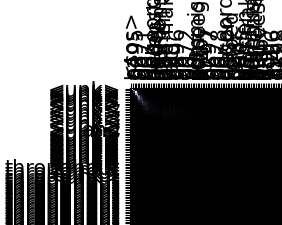
\includegraphics[width=0.4\linewidth]{figs/overalle.png}
    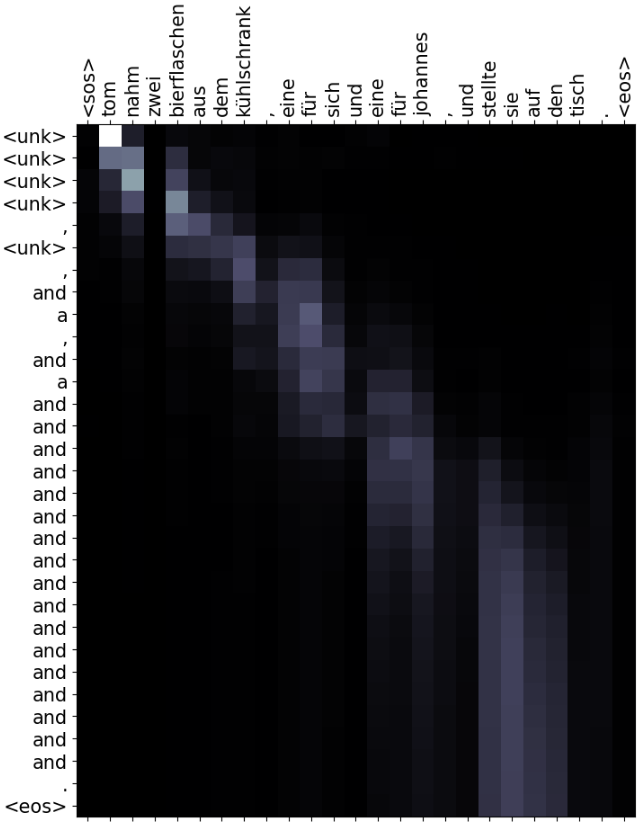
\includegraphics[width=0.4\linewidth]{figs/overallm.png}
    \caption{Attention maps of high overall word counts. Left attention is generated from the extreme test. Right attention is generated from the manageable.}
\end{figure}

If we compare this with examples of both the datasets for high unique word counts and attention maps in Figure 6, we can see that the more unique words had a low overall word count and had shorter input examples. 
\begin{center}
\begin{tabular}{p{2.5in}}
    Extreme stress test example:\\
    \hline
    these people are not holding out a begging bowl - they are only asking for recognition that they have small landowning democracies in countries which have human rights and which protect workers' rights.\\
    \\
    these people hold what appears to be their hands, they are \verb|<unk>|, will \verb|<unk>|, they are will \verb|<unk>| and the the .\\
    \hline
\end{tabular}
\end{center}
\begin{center}
\begin{tabular}{p{2.5in}}
    Manageable stress test example:\\
    \hline
    How long can you stand on one leg with your eyes closed?\\
    \\
    this long - haired \verb|<unk>| with their eyes closed on a a stand, one of them.\\
    \hline
\end{tabular}
\end{center}
While there are still syntactical and semantic errors, the overall contextual understanding by the model was higher according to the attention map. Although it should be noted that in both attention matrices, we do see the same weight drop off in the later tokens. 
\begin{figure}
    \centering
    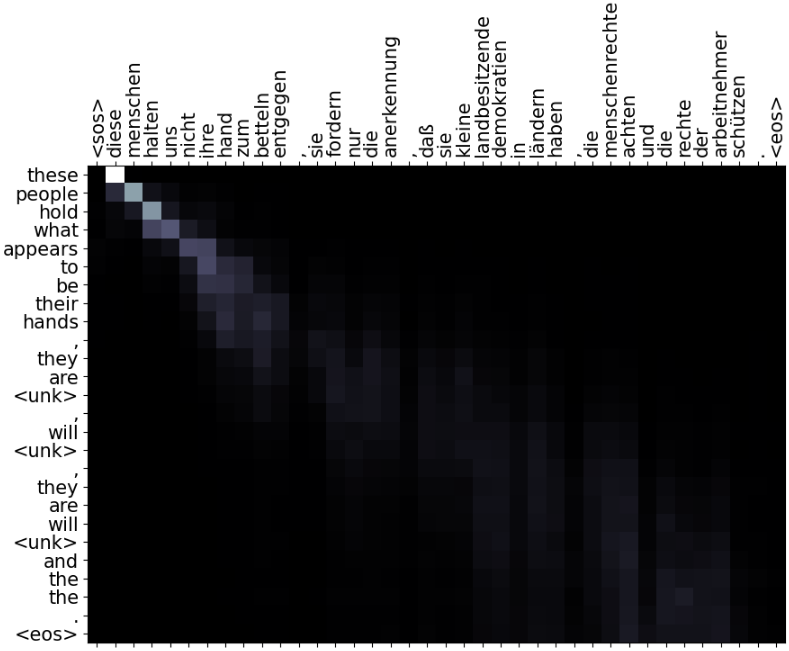
\includegraphics[width=0.4\linewidth]{figs/uniquee.png}
    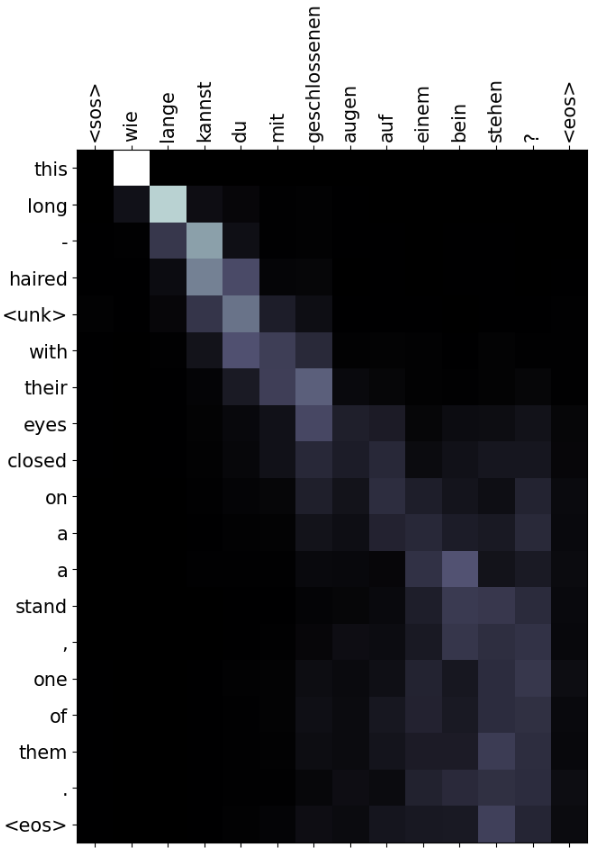
\includegraphics[width=0.4\linewidth]{figs/uniquem.png}
    \caption{Attention maps of high unique word counts. Left attention is generated from the extreme test. Right attention is generated from the manageable.}
\end{figure}

\subsection{Frequencies and Conditions}
The errors presented earlier were frequent and this conclusion can be obtained with stricter filters on the translations as shown in Figure 7. These filters allow us to observe two characteristics: how well was the model able to generate a known token and what conditions cause translations to fail these filters, and consequently perform poorly.
\begin{figure}[h]
    \centering
    \begin{tabular}{| l || c | c || c | c |}
    \hline
    Filter & E. Cnt. & E. \% & M. Cnt. & M. \%\\
    \hline
    \hline
    75\% & 111917 & 49\% & 228758 & 82\% \\
    50\% & 41926 & 18\% & 159789 & 58\%\\
    25\% & 11274 & 4.9\% & 85940 & 31\%\\
    0\% & 1428 & 0.62\% & 30203 & 11\%\\
    \hline
    \end{tabular}
    \caption{Number of translations (Cnt.) and percentage of all translations that passed each filter for the extreme (E.) and manageable (M.) stress dataset.}
\end{figure}

Applying a stricter filtration of $50\%$ and $75\%$--i.e. percentage of non-\verb|<unk>| tokens-- on the extreme stress results kept only $18\%$ and $5\%$ of the results, respectively. The same filters were applied to the manageable stress results and kept only $58\%$ and $31\%$ of the translations, respectively. Figure 7 shows the filters dropped the amount of results pseudo-exponentially with increasing strictness. This means that the model was struggling with the majority of the translations and producing a lot of \verb|<unk>| tokens.

A final filter for approximately zero \verb|<unk>| tokens was performed on both datasets, resulting in 1428 ($0.62\%$) translations of the extreme dataset and 30203 ($10.87\%$) translations of the manageable dataset. Two translations, one from each dataset, are shown with the attention maps in Figure 8:

\begin{center}
\begin{tabular}{p{2.5in}}
    Extreme stress test example:\\
    \hline
    the hotel is set in an acre of grounds and is comprised of 2 buildings.\\
    \\
    the is laying on the top of a heavily square , with several buildings and buildings.\\
    \hline
\end{tabular}
\end{center}
\begin{center}
\begin{tabular}{p{2.5in}}
    Manageable stress test example:\\
    \hline
    i have three dogs. One is male and the other two are female.\\
    \\
    this is three three dogs are a a toy in the other and two other men.\\
    \hline
\end{tabular}
\end{center}
While these are considered well-performing under the filter, they still have syntactic errors. Nonetheless, they performed relatively well in retaining the overall semantic of the sentence(s) and was able to mostly understand and maintain most of the original input's meaning.

\begin{figure}
    \centering
    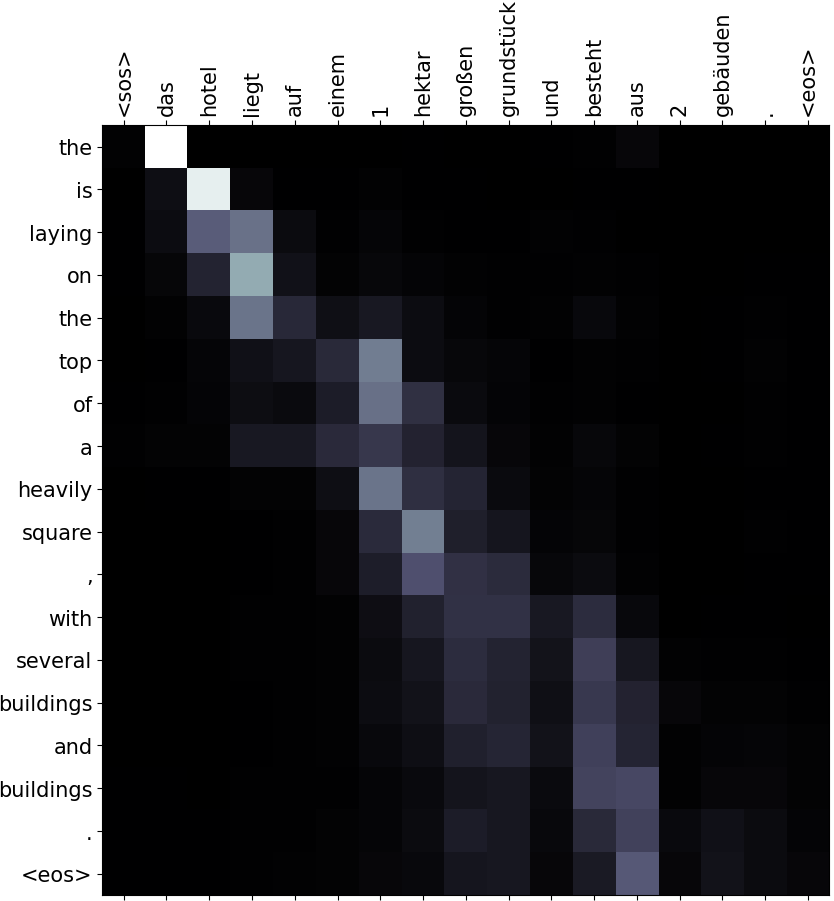
\includegraphics[width=0.4\linewidth]{figs/building_attention.png}
    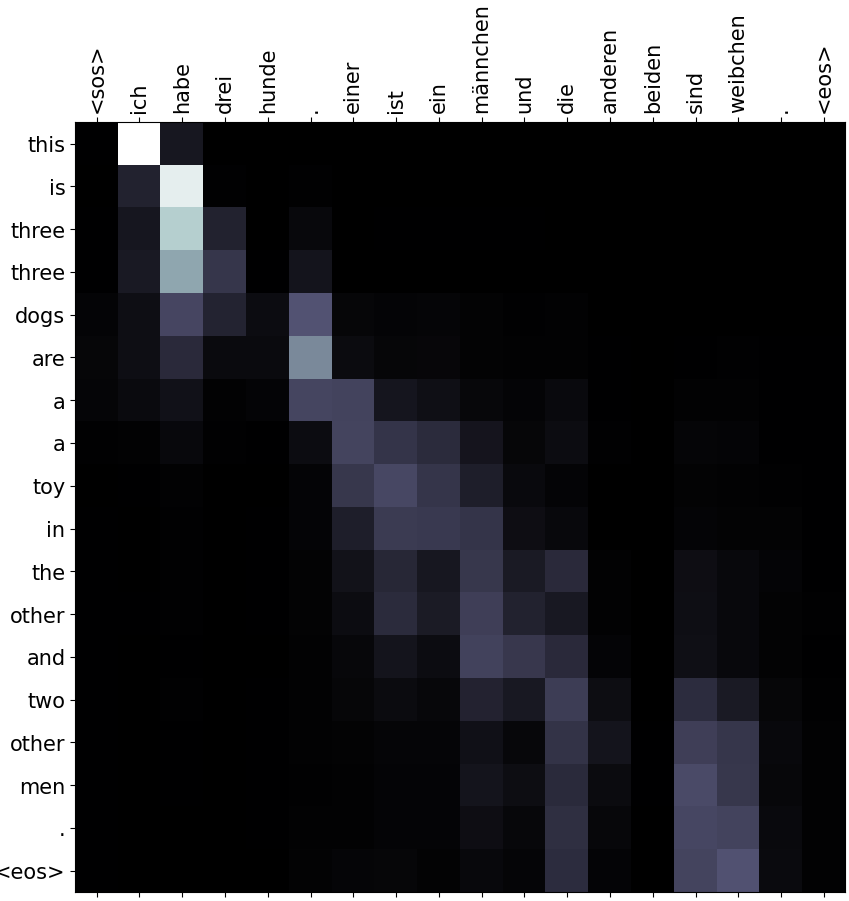
\includegraphics[width=0.4\linewidth]{figs/dog_attention.png}
    \caption{Attention maps of translations kept from the $0\%$ filter. Left attention is generated from the first translation about buildings. Right attention is generated from the second translation about dogs.}
\end{figure}

However, one commonality of these two sentences is that they are both short. In fact, all examples provided in the paper that performed somewhat well were short inputs that typically hovered within the 10-30 word range. As mentioned in the original filter, the manageable stress dataset required a filter bypass at the lowest strictness filter for complexity groups 3 and 4. This means that the model struggled to obtain or maintain any meaningful context from the longer German sentences. 

The $0\%$ filter also shows translation deterioration in respect to the example length only $2$ examples of the $30203$ remaining results were complexity 2, with the rest being complexity 1. Similarly as mentioned earlier, the extreme stress testing with much longer inputs had a much worse BLEU score than the shorter input manageable stress testing. Thus, the two conditions for these errors are likely both complex and long sentences.

% Present the errors found during the analysis, supported by specific examples. Categorize the types of errors encountered (e.g., syntactic errors, semantic misunderstandings, context misinterpretations, etc) and discuss their frequencies or conditions under which they appear.


\section{Discussion}
Before reviewing the results, some considerations must be made regarding the testing of each dataset. As mentioned earlier, the extreme test dataset contained longer entries with up to and around 1600 words. Meanwhile, the manageable stress dataset contained lower word counts. A reminder that both these dataset stress tests the model against possible real use cases of on-demand translations of entire webpages or passages with more realistic/human writing.

With the aforementioned considerations, we can consider that while the BLEU scores were poor, general translation performance was relatively good under stress conditions. Nonetheless, with all the results presented, it becomes clear that while the model does help with some longer sentences as stated in the paper \cite{bahdanau2016neural}, it still struggles and produces errors for others sentences, including some shorter ones. 

As mentioned in the translation examples, we typically see better performance with less sentences. Short sentences $<15$ words tend to perform the best, confirming that long sentence lengths were the main conditions for these errors. At the same time, we observed that the performance was best at the beginning for unfiltered longer sentences. This is largely due to how the attention model works. As it explores later tokens, it starts having issues maintaining context. While the GRU helps with improving long-term memory, it still fails with much longer sentences, which the original paper also mentioned as a possible issue. Moroever, the paper also demonstrated a deteriation of BLEU scores and performance as the input length increased \cite{bahdanau2016neural}.

The more complex, or realistic, examples likely pushed the model past its limits as it was trying to form relational mappings with more dynamic, complex or realistic, writings. While the model appears to obtain some meaning of the German inputs in the encoder, the decoder likely had issues generating and pairing these meanings with English words to form the same meaning, resulting in \verb|<unk>| tokens and the more "blurred" attention maps.

% Discuss your reasons as to why  you think these errors occur, possibly drawing on literature in NLP.  If applicable, compare your findings with those discussed in the literature.


\section{Looking Forward}
Based on the discussion, a few changes to the model can be made to deal with these difficult cases. The first major struggle of the model presented in this paper deals with complex realistic inputs. The most obvious solution would be to train the model on a much larger corpus of real text translation entries scraped from the internet. Websites that offer native de-en or any language translation accessibility may be good sources. 

Another approach for these cases may be to use LSTMs for the RNN layers. LSTMs use an input, output, forget gate, and memory cell state for infromation control in comparison to the GRU's more simple update and reset gate. The LSTM can assist the model in learning and retaining relevant relational details of more complex, dynamic human writings \cite{Srivatsavaya_2023}. 

Aside from changing the RNN block, adding more RNN layers can be another approach. The current encoder-decoder model presented in the paper uses only one GRU block in the encoder and decoder. Adding more blocks in the encoder may allow the model to find more details for dealing with the more complex inputs. Similarly, multiple GRU blocks in the decoder may help the model to apply the learned features from the encoder's attention mechanisms better. This idea draws on the architecture of Google's GNMT which uses multiple LSTM layers in the encoder and decoder \cite{wu2016googles}.

However, having more LSTM blocks may also pose an issue with information loss or exploding gradients. To address this, residual layers could be added in between every few recurrent layer to re-integrate previous information. A visual learning ResNet can be used as a reference due to its high performance with image identification tasks \cite{he2015deep}. Testing will need to be done to find the optimal placement of each residual layer. Google's GNMT suggests placing a residual between each LSTM layer; however, spacing the residual layer out may help in providing the model with more learning capacity of newer details.

Finally, another change could be to perform chunk learning of the words of the longer sentences. One major issue noted in stress tests was the difficulty with providing relational weights in the attention map of later tokens. Splitting long inputs into chunks and learning from individual segments may allow the model to generate better attention maps. These attentions can be re-pooled and tuned against the full input to compute the main larger attention that can be used to map the relations of translated tokens. This suggestion is similar to the attention-over-attention mechanism used for summary generation \cite{Cui_2017}.

% How can the difficult cases you identified be addressed? Outline what changes in terms of data, models, algorithms, or evaluation metrics are necessary to resolve these issues. Develop a comprehensive plan for improving the system's performance.

\section{Conclusion}
This survey tested the seq2seq attention-based GRU encoder-decoder model against extreme inputs. The attention mechanism helped with allowing the NMT in translating sentence lengths between 15-20 words and even up to 50 words with a larger training dataset. However, the results of this survey has found the model to be prone to errors as it struggles to provide accurate translations of longer inputs, which may be a requirement for real use cases of large passage translations. 

Stress tests with complex inputs revealed additional struggles of the model with irregular inputs. Complex inputs were any examples that contained more realistic text translations that may mimic the more dynamic writings that people may produce. Some other typs may also include non-conversational or texts meant to have no meaning, such as acknowledgements or citations. This may make translating blogs or academic papers all at once difficult and error prone. Future changes suggested in this survey may help the attention-RNN NMT model to perform better with both longer sentences and more complex inputs such as those used in the stress tests.

While the model faced difficulties with the longer and complex examples, translation of smaller inputs were shown to not be perfect either. Contextual misunderstandings and errors with syntactic generations were common across inputs of varying lengths. Nonetheless, the model was capable of learning most of the surrounding meanings due to its attention model, allowing it to perform better than basic SMT models. 


% Recap the major findings  from the analysis.
% State the implications of the implications of your findings.


\section{Acknowledgements}
ChatGPT was only used for the following areas in the \textbf{Introduction} section for proofreading: (1) "MT tools \st{have primarily been utilized to translate}" $\rightarrow$ "MT tools \textit{primarily translated}", (2) "KyungHyun Cho et al. reveal\st{s}" $\rightarrow$ "KyungHyun Cho et al. reveal\textit{ed}", (3) italicization of the title for Bahdanau's paper, and (4) punctuation. Other sections were not passed into ChatGPT due to the volume of text.

These resources were used to help understand some of the papers referenced in this survey: \textit{Understanding GRU Networks from Medium} \cite{Kostadinov_2019} and \textit{LSTM vs GRU from Medium} \cite{Srivatsavaya_2023}.

The codebase that was used was derived from a tutorial implementation of the official seq2seq PyTorch module \cite{github}. The original model was kept as is with additional datasets and code implementations to stress test the mode. My implementation can be found at https://github.com/PikaSannnnn/CSE256-Literature-Survey-and-Proposal/tree/main.

% Generative AI tools such as ChatGPT, Bard, DALL-E,  Stable Diffusion,  and Copilot  have applications that help student learning and understanding, however, these tools can also be used in ways that bypass key learning objectives.

% For this reason, using generative AI tools to substantially complete your report  is not permitted (i.e. you can't just have ChatGPT write your entire report for you).
% You are allowed to use these tools as general-purpose assistants such as proof-readers, etc. When you use these tools, please disclose relevant use-cases in your report and specify in this section:
% \begin{itemize}
% \item  The degree to which you changed the outputs of the tool (no changes, minor changes, or major changes)
% \end{itemize}


\bibliographystyle{apalike}
\footnotesize
\bibliography{references}



\end{document}
